\documentclass{article}
% Útgáfa 1.5

% pakkar fyrir töflur; array er notað í "math-mode"; arydshln fyrir brotalínur í töflum
\usepackage{array,tabularx}%,arydshln}  
% íslenskt letur, orðaskiptingar ...
\usepackage[english]{babel}
\usepackage[T1]{fontenc}
% númera jöfnur, töflur, myndir, ...
\usepackage{enumerate}
% fyrir krækjur
\usepackage[colorlinks,linkcolor=blue,citecolor=blue,urlcolor=blue]{hyperref}
% ýmis tákn, leturgerðir, ... ATH amsmath fyrir \text{} skipunina
\usepackage{amsmath,amssymb,euscript}   
% til að setja inn *.eps myndir ef við notum dvi og ps skjöl...
\usepackage{epsfig}    % \epsfig{...}
% ... en ef við notum pdf beint, þá er þetta pakkinn sem við þurfum
\usepackage{graphicx}  % \includegraphics[...]{...}
% litamöguleikar fyrir texta
\usepackage{color}
% til þess að myndir og töflur standi þar sem þær eiga að standa!
\usepackage{here}
%
\setlength{\textwidth}{7in}
\setlength{\textheight}{9in}
\setlength{\headheight}{0in}
\setlength{\headsep}{6pt}
\setlength{\topskip}{0in}
\setlength{\topmargin}{0cm}
\setlength{\oddsidemargin}{-0.3in}
\setlength{\marginparwidth}{10pt}
% dregur fyrstu línu í hverri málsgrein inn - nota 0cm fyrir engan inndrátt fyrir allar málsgreinar en \noindent í upphafi málsgreinar til að hafa engan inndrátt í þeirri málsgrein einni:
\setlength{\parindent}{0cm}
% viljum hafa eitt línubil milli efnisgreina
\setlength{\parskip}{1.5ex plus 0.75ex minus 0.5ex}
% 1.5 í línubil
\renewcommand{\baselinestretch}{1.025}

% Environments
\newenvironment{alist}[1][$\quad\,$1.]{
\vspace*{-8pt} \begin{enumerate}[label=\alph*),itemsep=4pt,parsep=3pt]}
{\end{enumerate}\vspace*{-3pt}}

\newenvironment{ttafla}[1][$\quad\,$1.]{
\begin{tabular}{rcl} \renewcommand\arraystretch{2} }
{\end{tabular}}



%Bætt við af mér (Hannesi)
% Þjappa saman
\widowpenalty=600
\clubpenalty=600
\usepackage[compact]{titlesec}
\titlespacing{\section}{0pt}{2ex plus 0.75ex minus 0.75ex}{1ex plus 0.3ex minus 0.3ex}
\titlespacing{\subsection}{0pt}{1ex plus 0.25ex minus 0.25ex}{0ex plus 0.1ex minus 0.1ex}
\titlespacing{\subsubsection}{0pt}{0.5ex plus 0.1ex minus 0.1ex}{0ex plus 0.1ex minus 0.1ex}

% Bolda caption
\usepackage[hang,small,bf]{caption}

% Efnaformúlur og myndir
%\usepackage[version=3]{mhchem}
\usepackage{chemfig}

% Komma í stað punkts
\usepackage{icomma}

% Annað
\usepackage{subfig}
\usepackage{array}
\usepackage{bigstrut}
\usepackage{multirow}
\usepackage{multicol}
\usepackage{enumerate}
%\usepackage{enumitem}
\usepackage{wrapfig}
\newcommand{\HRule}{\rule{\linewidth}{0.5mm}}
\usepackage{ulem}
%\usepackage[thinspace,mediumqspace,amssymb]{SIunits}

%Tikz
\usepackage{tikz}
\usetikzlibrary{fit,arrows,decorations.pathmorphing,decorations.text,backgrounds,positioning,fit,petri,3d,calc}
%% 3d hnitakerfi
\usepackage{tikz-3dplot}
\tdplotsetmaincoords{75}{130}
%\begin{tikzpicture}[scale=5,tdplot_main_coords]
%
%%set up some coordinates 
%%-----------------------
%\coordinate (O) at (0,0,0);
%
%%determine a coordinate (P) using (r,\theta,\phi) coordinates.  This command
%%also determines (Pxy), (Pxz), and (Pyz): the xy-, xz-, and yz-projections
%%of the point (P).
%%syntax: \tdplotsetcoord{Coordinate name without parentheses}{r}{\theta}{\phi}
%\tdplotsetcoord{P}{\rvec}{\thetavec}{\phivec}


%%%%%%%%%%%%%%% SKIPANIR %%%%%%%%%%%%%%%%%%%%%%%%
%% LITASTYTTINGAR
%
\definecolor{dgreen}{rgb}{0,0.8,0}
\newcommand{\red}[1]{{\color{red} #1}}
\newcommand{\green}[1]{{\color{dgreen} #1}}
\newcommand{\blue}[1]{{\color{blue} #1}}
\newcommand{\black}[1]{{\color{black} #1}}
%
% ALLS KYNS STÆRÐFRÆÐIDÓT
%
\newcommand{\lvec}{\overrightarrow}
%
% ýmsar diffurstyttingar
\newcommand{\dif}{\,\mathrm{d}}
\newcommand{\dx}{\,\mathrm{d}x}
\newcommand{\dy}{\,\mathrm{d}y}
\newcommand{\dz}{\,\mathrm{d}z}
\newcommand{\dt}{\,\mathrm{d}t}
% afleiður og hlutafleiður
\renewcommand{\d}[2]{\frac{\dif{#1}}{\dif{#2}}}
\newcommand{\dd}[3]{\frac{\dif^{#1}{#2}}{\dif^{#1}{#3}}}
\newcommand{\p}[2]{\frac{\partial{#1}}{\partial {#2}}}
\newcommand{\pp}[3]{\frac{\partial^{#1}{#2}}{\partial{#3}^{#1}}}
%
% bil, millistig \; og \quad
\newcommand{\bil}{\hspace*{6pt}}
\newcommand{\Bil}{\hspace*{10pt}}
\newcommand{\vbil}{\vspace*{-6pt}}
\newcommand{\vBil}{\vspace*{-10pt}}

% samasemmerki með aukaplássi á báða bóga
\newcommand{\bils}{\bil=\bil}
%
\newcommand{\bc}{\begin{center}}
\newcommand{\ec}{\end{center}}
%
\newcommand{\beq}{\begin{equation}}
\newcommand{\eeq}{\end{equation}}
%
\newcommand{\beqa}{\begin{eqnarray*}}
\newcommand{\eeqa}{\end{eqnarray*}}
%
\newcommand{\ba}{\begin{array}}
\newcommand{\ea}{\end{array}}
%
\newcommand{\bma}{\begin{matrix}}
\newcommand{\ema}{\end{matrix}}
%
\newcommand{\bmh}{\left[\begin{matrix}}
\newcommand{\emh}{\end{matrix}\right]}
%
\newcommand{\ts}{\textstyle}
\newcommand{\ds}{\displaystyle}

% Frá mér (Hannesi)
\newcommand{\lausn}{\textbf{\textit{Lausn:}}}
\newcommand{\solution}{\textbf{\textit{Solution:}}}
\newcommand{\daemi}{\textbf{\textit{Dæmi:}}}
\newcommand{\bt}{\begin{table}[H]}
\newcommand{\et}{\end{table}}
\newcommand{\atm}{\text{atm}}
\newcommand{\calories}{\text{cal}}
\everymath{\displaystyle} % Svo allar jöfnur taka aldrei minna pláss
\renewcommand\tabcolsep{2pt} % Bil dalka í töflum
\setlength{\arraycolsep}{1.5pt}
%\usepackage{fancyhdr}
%\setlength{\headheight}{25pt}
%\pagestyle{fancy}
%\renewcommand{\headrulewidth}{0.4pt}
%\renewcommand{\footrulewidth}{0.4pt}
%\usepackage[top=2.5in, bottom=1.5in, left=1in, right=1in]{geometry}
\usepackage{amssymb}
\usepackage{pifont}
\newcommand{\cmark}{\text{\ding{51}}}%
\newcommand{\xmark}{\text{\ding{55}}}%

\usepackage{pbox}
%\usepackage{fancyvrb}
\usepackage{array}
\newcolumntype{L}[1]{>{\raggedright\let\newline\\\arraybackslash\hspace{0pt}}m{#1}}
\newcolumntype{C}[1]{>{\centering\let\newline\\\arraybackslash\hspace{0pt}}m{#1}}
\newcolumntype{R}[1]{>{\raggedleft\let\newline\\\arraybackslash\hspace{0pt}}m{#1}}
\usepackage[utf8]{inputenc}
\usepackage{framed}
\usepackage{paralist}
\renewenvironment{enumerate}[1]{\begin{compactenum}#1}{\end{compactenum}}
\usetikzlibrary{shapes.multipart,positioning,arrows}

\begin{document}
\begin{titlepage}
\begin{center}
\textsc{}\\[2cm] 

\includegraphics[width=6cm]{Haskoli_Islands_rett.jpg}\\[0.5cm]
\HRule \\[0.6cm]
{ \huge \bfseries Group assignment 4: Refined OO model}\\[0.2cm]
\HRule \\[0.4cm]
\textsc{\normalsize Þróun hugbúnaðar} \\
\textsc{Spring 2015} \\[1.5cm]
\begin{minipage}{0.45\textwidth}
\begin{flushleft} \large
\textit{Students:} (Group F2a)\\
\textsc{Einar Helgi Þrastarson} \\
\textsc{Hannes Pétur Eggertsson} \\
\textsc{Sigurður Birkir Sigurðsson} \\
\end{flushleft}
\end{minipage}
\begin{minipage}{0.45\textwidth}
\begin{flushright} \large
\textit{Teachers:} \\
\textsc{Matthias Book}\\
\textsc{Kristín Fjóla Tómasdóttir}\\
\textsc{ }\\
\end{flushright}
\end{minipage}

\end{center}
\end{titlepage}


% Description of the project
\section{Introduction}
In this document there's the class diagram for group F2a. Group members are: Einar Helgi Þrastarson (personal ID number: 110287-2919), Hannes Pétur Eggertsson (240889-2939) and Sigurður Birkir Sigurðsson (120589-2539). Our project is to build an user interface for a fantasy football game. In our class diagram we felt it made sense to split the classes into two categories, back-end classes and front-end classes. Then, in a third diagram there's another diagram that shows the connections between the back-end and  We will all present this document on Wednesday, March ?th 2015.

\subsection{Notation}
In our class diagrams we use the following notation:\vspace*{-0.3cm}
\begin{itemize}\itemsep-4pt
\item[--] means a private variable or method (not directly accessable by other classed).
\item[+] means a public variable or method (directly accessable by other classes).
\end{itemize}

\tikzset{umlclass/.style={
        draw=black,fill=yellow!16,rectangle split,align=center, rectangle split part align={center,left}, minimum width=4cm,rounded corners},draw,rectangle split parts=4}

Each class in the diagram has four sections shown below:
\begin{center} \vspace*{-0.15cm}
\begin{tikzpicture}
\begin{scope}[xshift=8cm,yshift=0cm]
\node[umlclass] (t1)
 {\textbf{\large \textit{The class' name.}}
 \nodepart{two}
  {\footnotesize
  \begin{tabular}{l} 
   Short description of the class.
  \end{tabular}}
 \nodepart{three}
  \begin{tabular}{l}
  The class' variables and their type listed\\
  on the format:\\
   --/+ \texttt{type1 variable1}\\
   --/+ \texttt{anotherClass variable2}\\
  \end{tabular}
 \nodepart{four}
  \begin{tabular}{l}
   The class' methods listed on the format:\\
   --/+ \texttt{type1 method1(type variable,...)}\\
   --/+ \texttt{type2 method2(...)}\\
  \end{tabular}
 };
\end{scope}
\end{tikzpicture}
\end{center}\vspace*{-0.15cm}
If the class wasn't created by us it is filled with red. Classes are then interconnected using 3 types of arrows:

\begin{tikzpicture}
\draw[arrows={-angle 60},thick] node[left]{Class A} (0,0) to (3,0)node[draw=none,midway,above=0cm] {\hspace*{3cm}\textit{uses}} node[right]{Class B};
\begin{scope}[yshift=-0.8cm]
\draw[arrows={-open triangle 60},thick] node[left]{Class A} (0,0) to (3,0)node[draw=none,midway,above=0cm] {\hspace*{3cm}\textit{extends}} node[right]{Class B};
\end{scope}
\begin{scope}[yshift=-1.6cm]
\draw[arrows={-triangle 60},thick] node[left]{Class A} (0,0) to (3,0)node[draw=none,midway,above=0cm] {\hspace*{3cm}\textit{implements}} node[right]{Class B};
\end{scope}
\end{tikzpicture}

In most cases we can tell how many classes 'Class A' and 'Class B' will be associated with, this is shown by placing an arrow at the beginning and end of an arrow, e.g.

\begin{tikzpicture}
\draw[arrows={-angle 60},thick] node[left]{Class A} node[above right]{1} (0,0) to (3,0)node[draw=none,midway,above=0cm] {\hspace*{3cm}\textit{uses}} node[above left]{0--10} node[right]{Class B};
\end{tikzpicture}

if each instance of 'Class A' will use 'Class B' in a range of 0 to 10 instances.

\section{Class diagram}
We decided to split our class diagram into two figures: \textbf{Back-end classes} and \textbf{Front-end classes}. The back-end classes take care of storing and keeping track of all information as the game is running. The front-end classes take care of displaying the information to the users playing the game as well as handling their input.

\subsection{Back-end classes}
\begin{tikzpicture}
%% ==========================================
%% User
%% ==========================================
\begin{scope}[yshift=1cm]
\node[umlclass] (user)
 {\textbf{\large \textit{User}}
 \nodepart{two}
  {\footnotesize
  \begin{tabular}{l} 
   This class keeps track of all information about\\
   each user playing the game.\\
   
  \end{tabular}}
 \nodepart{three}
  \begin{tabular}{l}
   -- \texttt{int id}\\
   -- \texttt{int money}\\
   -- \texttt{int score}\\
   -- \texttt{int roundscore}\\
   -- \texttt{String name}\\
   -- \texttt{Roster roster}\\
  \end{tabular}
 \nodepart{four}
  \begin{tabular}{l}
   + \texttt{User(String name, int id)}\\
   + \texttt{int getMoney()}\\
   + \texttt{boolean isAffordable(int price)}\\
   + \texttt{void changeMoney(int dMoney)}\\
   + \texttt{Roster getRoster()}\\
   + \texttt{int getScore()}\\
   + \texttt{int getRoundScore()}\\
   + \texttt{void setScore(int newscore)}\\
   + \texttt{String getName()}\\
   + \texttt{void setName(String newname)}\\ 
  \end{tabular}
 };
\end{scope}

%% ==========================================
%% Roster
%% ==========================================
\begin{scope}[xshift=10cm,yshift=0.1cm]
\node[umlclass] (roster)
 {\textbf{\large \textit{Roster}}
 \nodepart{two}
  {\footnotesize
  \begin{tabular}{l} 
   Keeps track of which football players are in which user team/roster.
  \end{tabular}}
 \nodepart{three}
  \begin{tabular}{l}
   -- \texttt{List<Player> goalkeepers}\\
   -- \texttt{List<Player> goalkeepersOnField}\\
   -- \texttt{List<Player> defenders}\\
   -- \texttt{List<Player> defendersOnField}\\
   -- \texttt{List<Player> midfielders}\\
   -- \texttt{List<Player> midfieldersOnField}\\
   -- \texttt{List<Player> forwards}\\
   -- \texttt{List<Player> forwardsOnField}\\
   -- \texttt{int numberOfPlayersOnField}\\
  \end{tabular}
 \nodepart{four}
  \begin{tabular}{l}
   + \texttt{Roster()}\\
   + \texttt{int getNumberOfPlayersOnField()}\\
   + \texttt{boolean removePlayerFromField(Player player)}\\
   + \texttt{void removePlayerFromRoster(Player player)}\\
   -- \texttt{void removePlayer(Player p, boolean fromRoster)}\\
   + \texttt{boolean addPlayerToField(Player player)}\\
   + \texttt{boolean addPlayerToRoster(Player player)}\\
   + \texttt{List< List<Player> > getPlayersInRoster()}\\
   + \texttt{List< List<Player> > getPlayersOnField()}\\
   + \texttt{boolean isInRoster(Player player)}\\
   + \texttt{boolean isOnField(Player player)}\\
  \end{tabular}
 };
\end{scope}

%% ==========================================
%% MainGame
%% ==========================================
\begin{scope}[yshift=-7.68cm]
\node[umlclass] (maingame)
 {\textbf{\large \textit{MainGame}}
 \nodepart{two}
  {\footnotesize
  \begin{tabular}{l} 
   The main back-end class. Keeps track of\\
   the state of the game. It exists always\\
   while the game is running.
  \end{tabular}}
 \nodepart{three}
  \begin{tabular}{l}
   -- \texttt{static final MainGame game}\\
   -- \texttt{StatsHistory stats}\\
   -- \texttt{List<User> users}\\
   -- \texttt{int round}\\
   -- \texttt{int currentUser}\\
  \end{tabular}
 \nodepart{four}
  \begin{tabular}{l}
   -- \texttt{static MainGame()}\\
   + \texttt{MainGame getInstance()}\\
   + \texttt{void resetGame()}\\
   + \texttt{void setNumUsers(int num)}\\
   + \texttt{void nextUser()}\\
   + \texttt{int getRound()}\\
   + \texttt{List<User> getUsers()}\\
   + \texttt{StatsHistory getStatsHistory()}\\
   + \texttt{User getCurrentUser()}\\
   + \texttt{int getCurrentUserID()}\\
  \end{tabular}
 };
\end{scope}

%% ==========================================
%% Player
%% ==========================================
\begin{scope}[xshift=8cm,yshift=-6.6cm]
\node[umlclass,rectangle split parts=2,fill=red!32] (player)
 {\textbf{\large \textit{Player} <<interface>>}
 \nodepart{two}
  {\footnotesize
  \begin{tabular}{l} 
   This class will be made by group F1a.\\
   Each instance will contain information\\
   about a football player.\\
  \end{tabular}}
 \nodepart{three}
 \nodepart{four}
 };
\end{scope}

%% ==========================================
%% StatsHistory
%% ==========================================
\begin{scope}[xshift=10cm,yshift=-13cm]
\node[umlclass] (statshistory)
 {\textbf{\large \textit{StatsHistory}}
 \nodepart{two}
  {\footnotesize
  \begin{tabular}{l} 
   A class that has statistical information.
  \end{tabular}}
 \nodepart{three}
  \begin{tabular}{l}
   -- \texttt{List<ObjectScores> allplayerscores}\\
   -- \texttt{List<ObjectScores> alluserscores}\\
   -- \texttt{List<ObjectScores> allrosterscores}\\
  \end{tabular}
 \nodepart{four}
  \begin{tabular}{l}
  + \texttt{StatsHistory()}\\
  + \texttt{void createPlayerScoreObject(Object player)}\\
  + \texttt{void createUserScoreObject(Object user)}\\
  + \texttt{void createRosterScoreObject(Object roster)}\\
  + \texttt{List<Integer> getPlayerScores(Player player)}\\
  + \texttt{List<Integer> getUserScores(User user)}\\
  + \texttt{void addScoreToPlayer(Player player, int score)}\\
  + \texttt{void addScoreToUser(User user, int score)}\\
  \end{tabular}
 };
\end{scope}

%% ==========================================
%% PlayerScores
%% ==========================================
\begin{scope}[xshift=0cm,yshift=-14.5cm]
\node[umlclass] (playerscores)
 {\textbf{\large \textit{ObjectScores}}
 \nodepart{two}
  {\footnotesize
  \begin{tabular}{l} 
   A class with information about each player.
  \end{tabular}}
 \nodepart{three}
  \begin{tabular}{l}
   -- \texttt{Object object}\\
   -- \texttt{List<Integer> scores}\\
   -- \texttt{List<Integer> totalscores}
  \end{tabular}
 \nodepart{four}
  \begin{tabular}{l}
   + \texttt{ObjectScores(Object object)}\\
   + \texttt{void addScore(int score)}\\
   + \texttt{List<Integer> getScores()}\\
   + \texttt{List<Integer> getTotalScores()}\\
   + \texttt{Object getObject()}
  \end{tabular}
 };
\end{scope}

%% ==========================================
%% Allar örvar teiknaðar hér
%% ==========================================
% user to roster
\draw[arrows={-angle 60},thick] ([yshift=-20pt]user.three east) node[right]{1} to [out=45, in=-150](roster.text west) node[above left]{1};

% maingame to user
\draw[arrows={-angle 60},thick]
[out=0, in=90](maingame.three east) node[right=0.15cm]{1} to [out=75, in=-75](user.text east) node[right]{1--N};

% maingame to statshistory
\draw[arrows={-angle 60},thick]
[out=0, in=90]([yshift=0.5cm]maingame.three east) node[right=0.15cm]{1} to [out=-65, in=111](statshistory.text west) node[left]{1};

% roster to player
\draw[arrows={angle 60-},thick] (player.text west) to [out=105, in=-120]([yshift=-1cm]roster.three west);

% StatsHistory to PlayerScores
\draw[arrows={-angle 60},thick] ([yshift=0.2cm]statshistory.three west) node[above left]{1} to [out=-135, in=10](playerscores.text east) node[below right]{$P$};

% StatsHistory to Player (backwards)
\draw[arrows={angle 60-},thick] ([yshift=0.2cm]statshistory.four west) to [out=110, in=-120](player.text west);
\end{tikzpicture}  
$N$ is er number of total users in the current game and $P$ is the total amount of football players in the game.

\newpage
\subsection{Front-end classes}
\begin{tikzpicture}
%% ==========================================
%% Main
%% ==========================================
\begin{scope}[xshift=0cm,yshift=0cm]
\node[umlclass] (main)
 {\textbf{\large \textit{Main}}
 \nodepart{two}
  {\footnotesize
  \begin{tabular}{l} 
   The main front-end class. It is initialized at\\
   the start of the game and runs until the game\\
   is terminated.
  \end{tabular}}
 \nodepart{three}
  \begin{tabular}{l}
   -- \texttt{static final Main instance}\\
   -- \texttt{JFrame frame}\\
   -- \texttt{JPanel right}\\
   -- \texttt{JPanel change}\\
   -- \texttt{MainGame game}\\
  \end{tabular}
 \nodepart{four}
  \begin{tabular}{l}
   -- \texttt{static Main()}\\
   + \texttt{static Main getInstance()}\\
   + \texttt{void startGame()}\\
   + \texttt{void restartFrame()}\\
   + \texttt{void setPanelAsMarket()}\\
   + \texttt{void setPanelAsScore()}\\
   + \texttt{void setPanelAsRoster()}\\
   + \texttt{void setPanelAsLeague()}\\ 
   + \texttt{void setPanelAsFieldViewer()}\\ 
   + \texttt{Dimension returnSizeForPanel()}\\
   + \texttt{static void main(String[] args)}\\
  \end{tabular}
 };
\end{scope}

%% ==========================================
%% Start Panel
%% ==========================================
\begin{scope}[xshift=0cm,yshift=0cm]
\node[umlclass] (Start Panel)
 {\textbf{\large \textit{Start Panel}}
 \nodepart{two}
  {\footnotesize
  \begin{tabular}{l} 
   Desc.
  \end{tabular}}
 \nodepart{three}
  \begin{tabular}{l}
   -- \texttt{JPanel center}\\
   -- \texttt{JTextField field}\\
   -- \texttt{List<String> names}\\
   -- \texttt{int numEmpty}\\
   -- \texttt{JButton startGame}\\
   -- \texttt{JButton addPlayer}\\   
  \end{tabular}
 \nodepart{four}
  \begin{tabular}{l}
   + \texttt{StartPanel()}\\
   + \texttt{addPlayerHandler()}\\
   + \texttt{void changeCenter()}\\
  \end{tabular}
 };
\end{scope}

%% ==========================================
%% generic template
%% ==========================================
%\begin{scope}[xshift=0cm,yshift=0cm]
%\node[umlclass] (generic)
% {\textbf{\large \textit{Generic}}
% \nodepart{two}
%  {\footnotesize
%  \begin{tabular}{l} 
%   Desc.
%  \end{tabular}}
% \nodepart{three}
%  \begin{tabular}{l}
%   -- \texttt{type var}\\
%  \end{tabular}
% \nodepart{four}
%  \begin{tabular}{l}
%   + \texttt{type method(type var)}\\
%  \end{tabular}
% };
%\end{scope}
\end{tikzpicture}

\newpage
\subsection{Connections between front-end and back-end classes}

\newpage
\section{Sequence diagrams}


\end{document}